% !TEX root = ../notes_template.tex

\chapter{Circulation}\label{chp:circulation}
Updated on \today
\minitoc
This chapter covers the circulation support of micro-circulation, which supports the ECF, which supports skeletal muscle function. Circulation includes two vascular circuits that circulates blood through the systemic and pulmonary circulation. The cardiac pump that supports circulation is covered in the next chapter.  

The primary goal of this chapter is an understanding of circulation in its supportive role for skeletal muscle. Circulation is critical for sustaining the micro-circulation of the ECF for cellular functions throughout the body. Without circulation cells with a high resting metabolism such as the brain and heart can only survive for minutes. The lack of $O_2$ delivery, and lack of $CO_2$ removal being the first two problems that threaten cell life. Problems with circulation can limit the metabolic function of muscles.   

The importance of circulation for life and function makes it a highly studied area of physiology. Since it has been highly studied it has several useful models for understanding circulation. After reviewing the important structures for circulation the chapter introduces several of the useful models (in the form of equations that demonstrate relationships).


\vspace{5mm}
\begin{svgraybox}
\textbf{Objectives include:}
\begin{enumerate}
    \item Describe how the anatomy of the heart and blood vessels supports circulation. 
    \item Identify cardiac anatomy structures.
    \item Explain and Interpret models (equations) of cardiac output, blood pressure and resistance.
    \item Apply equations of cardiac output, blood pressure and resistance (including Poiseuille's Law) to explain and evaluate the function and possible dysfunction of circulation.
    \item Explain circulation regulation based on blood pressure regulation.
    \item Explain blood pressure regulation.
    \item Interpret the events of vasovagal syncope.
    \item Explain the response of blood pressure to a graded exercise test.
    \item Explain systemic circulation including its distribution and cardiac index; cardiac circulation and pulmonary circulation.
    \item Perform and interpret cardiovascular tests and measures including: Heart rate and Blood pressure
\end{enumerate}
\end{svgraybox}

\section{Structures of Circulation}

The heart and the roots of the great vessels occupy the pericardium, which is located in the mediastinum. The sternum, the costal cartilages, and the medial ends of the third to fifth ribs on the left side of the thorax create the anterior border of the mediastinum. It is bordered inferiorly by the diaphragm, posteriorly by the vertebral column and ribs, and laterally by the pleural cavity (contains lungs). Specific cardiac structures and vessels are depicted in Figure \ref{fig:Cardiac_Anatomy}.

\begin{figure}[!h]
    \centering
    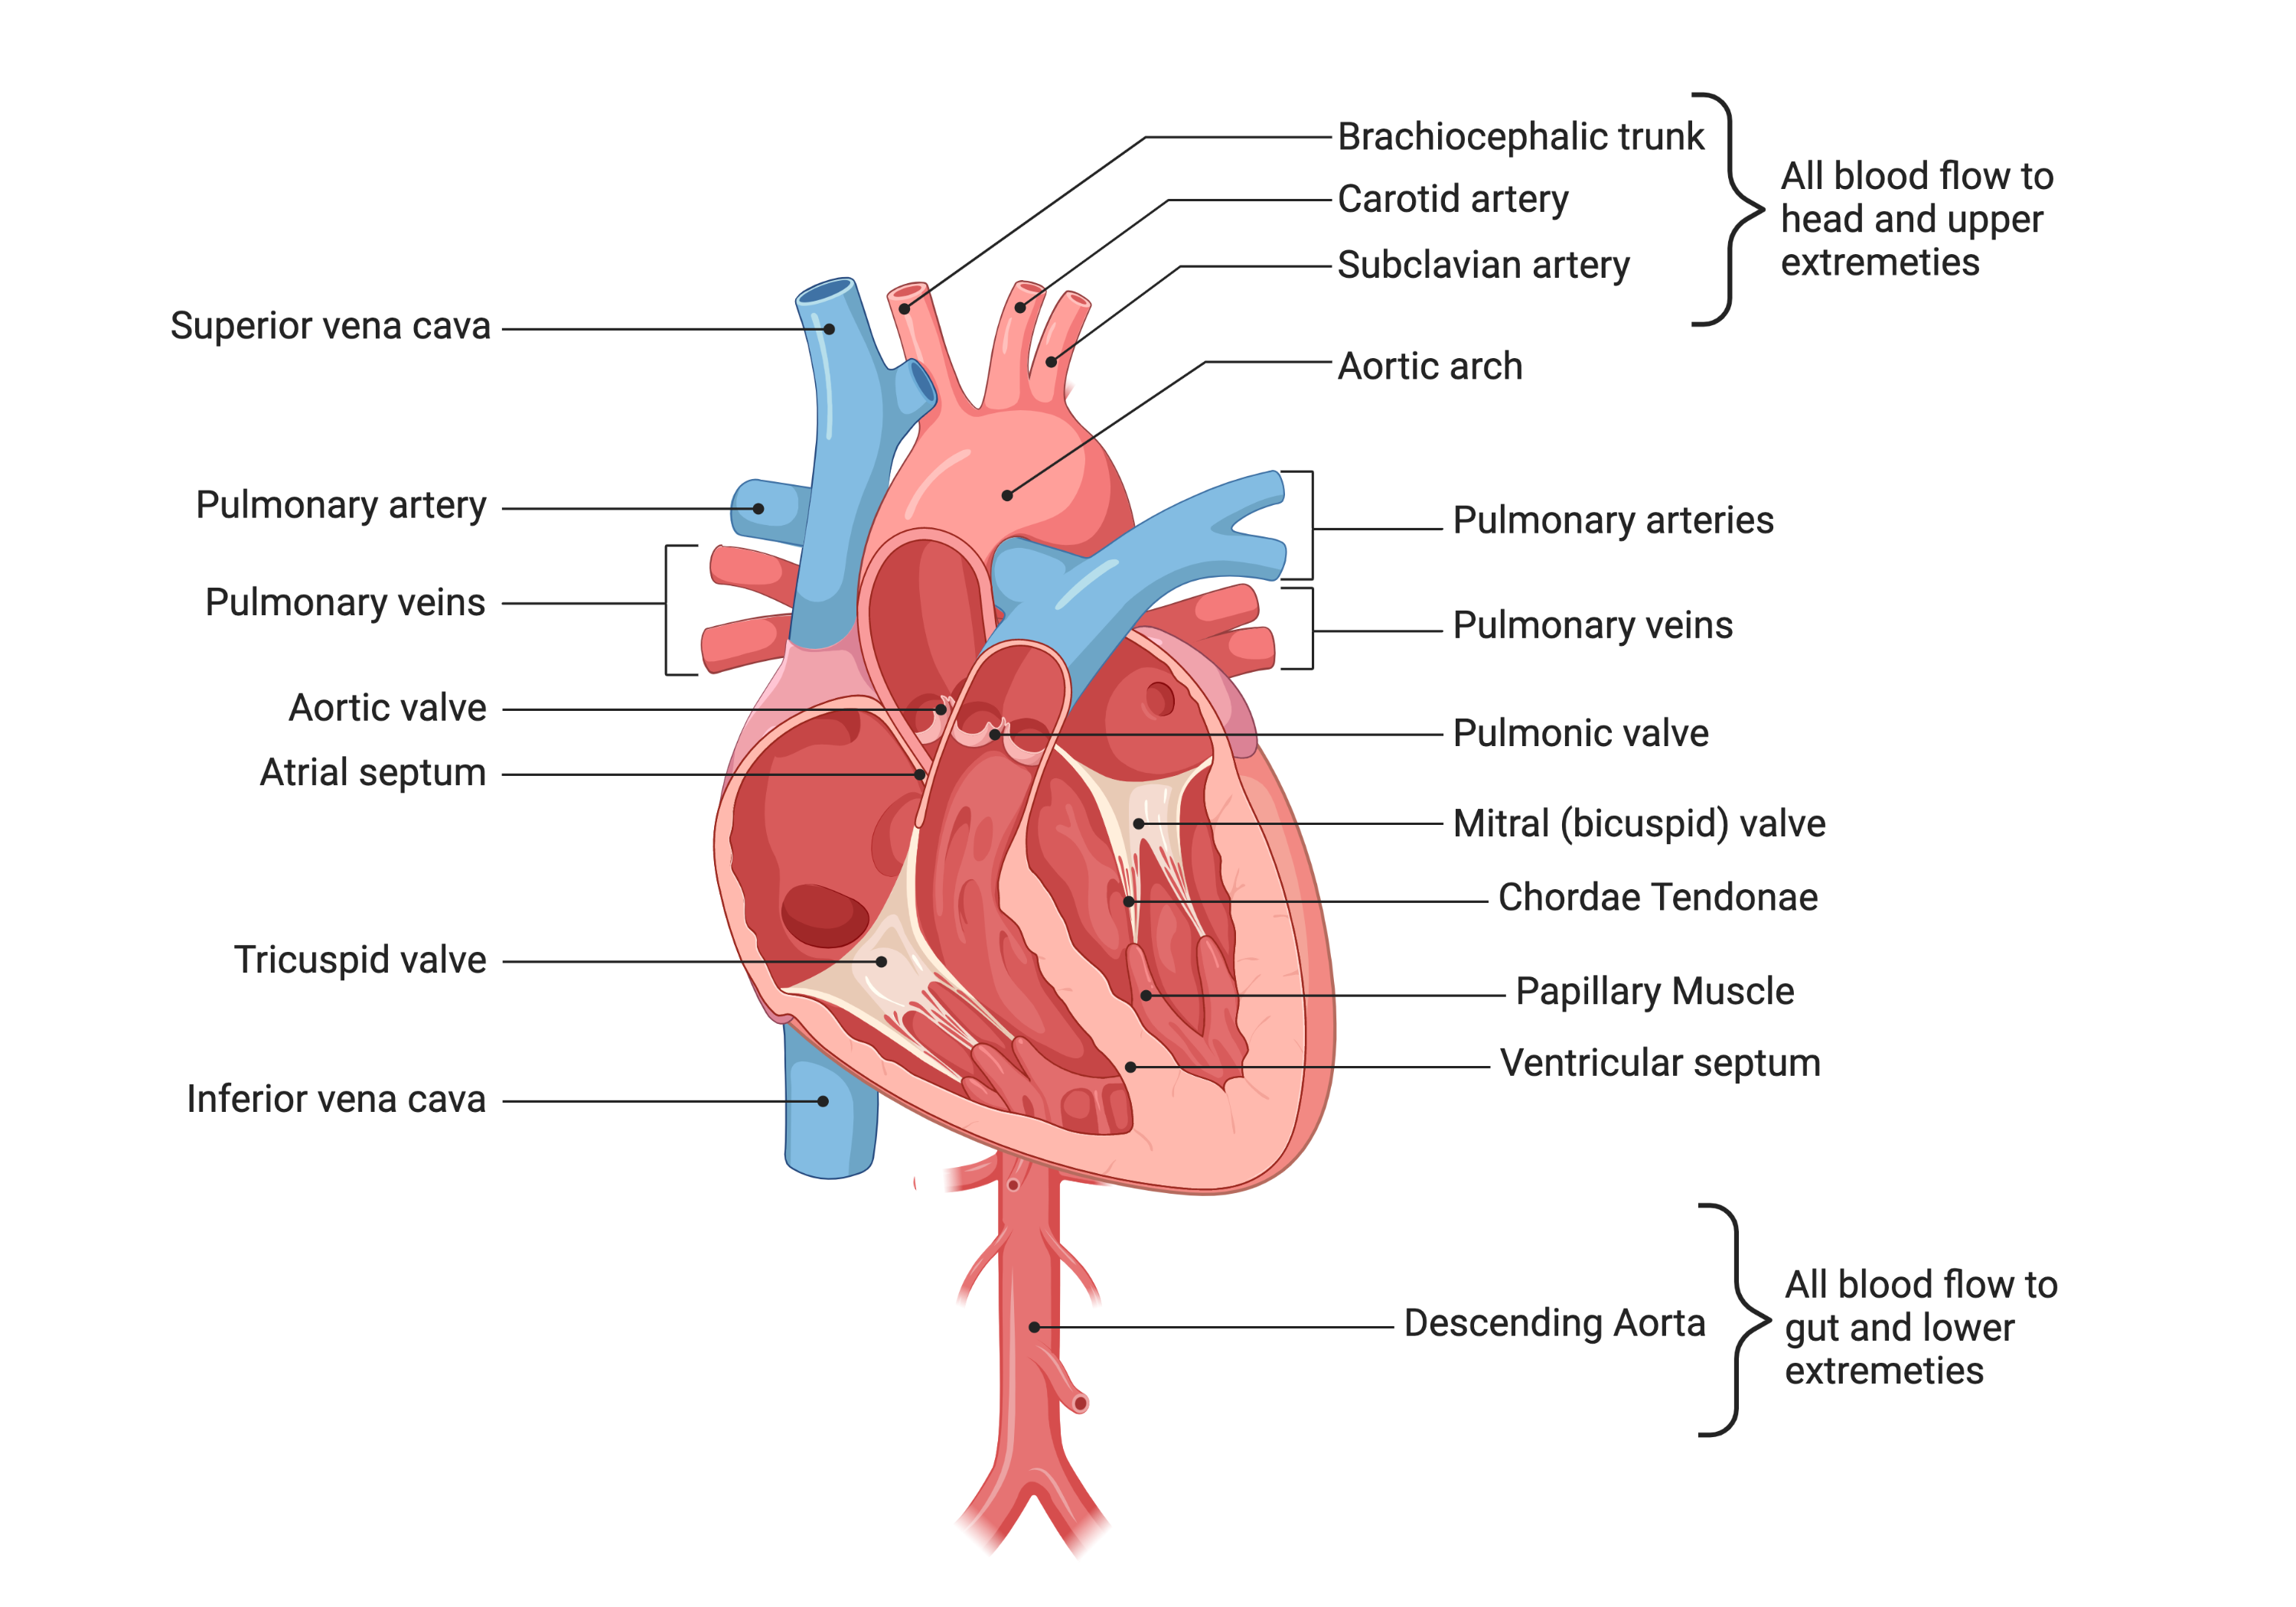
\includegraphics[width=1\linewidth]{./figure/Cardiac_Anatomy.png}
    \caption{Cardiac Anatomy \footnotesize{(Created with BioRender.com)}}
    \label{fig:Cardiac_Anatomy}
\end{figure}

Beyond being familiar with the structure in Figure \ref{fig:Cardiac_Anatomy} that are utilized throughout the chapter, there are several important structural takeaways.

\begin{itemize}
    \item Structurally there are four chambers, right and left atria (RA and LA); right and left ventricle (RV and LV) (the anatomical view).
    \item The four chambers form two primer-pumps for two circulations (right and left), RA and RV for the pulmonary circulation; and LA and LV for the systemic circulation (which includes all skeletal muscles and the heart itself) (the pump view).
    \item Cardiac muscle (myocardium) is thicker in the ventricles than the atria; and on the left side than the right side.
    \item The four chambers are divided into two excitation regions, RA and LA for atrial excitation; and RV and LV for ventricular excitation (the excitation view).
    \item The amount of tension and excitation is related to the thickness of the myocardium; which is based on how much pressure that chamber must generate for circulation.
    \item Circulation between the right and left primer-pumps is prevented by a septum (septal wall), also myocardium, that is thinner than the outer myocardial wall; and also thicker in the ventricles than the atria.
    \item Circulation direction is guided by four one-way valves. Circulation occurs due to pressure gradients - there is nothing inherently directional about pressure gradients other than high pressure to low pressure - therefore the valves are necessary to keep blood flowing from a chamber to the next chamber and now "backwards".
    \item All circulation from the gut and lower extremity passes through the descending aorta; and comes to the heart through the inferior vena cava.
    \item All circulation from the upper extremities and head passes through the great vessels (first three branches off of the aorta); and comes to the heart from the superior vena cava.
    \item For blood to flow through the circulation, venous pressure must be lower than arterial pressure
    \item Venous pressure (systemic in the RA; pulmonary in the LA) refers to the pressure that is the final end point for all venous circulation returning to the heart which must, for circulation to occur, have the lowest venous blood pressure of the respective circulations ($P_{RA} = 0$ when the RA is not generating tension). \item Ventricular systolic pressure refers to the pressure in the ventricles during active tensioning (contraction), for circulation to occur it must have the highest arterial pressure of the respective circulations. The right sided ventricular systolic pressure is lower than the left sided ventricular systolic pressure, the respective circulations are considered low and high pressure.
    \item Because the ventricular systolic pressures must be the highest through the circulation, the tricuspid valve (between the RA and RV) and the bicuspid (mitral) valve (between the LA and LV) have additional support supplied by the papillary muscles and chordae tendonae (the support does not help them open, it prevents them from allowing backflow while closed).
    \item Because the LV has greater pressure than the RR, the mitral valve papillary muscle and chordae tendonae are more developed
    \item The aortic valve, which is not supported by papillary muscle, is under more pressure than the tricuspid valve because the aortic pressure is the second highest pressure in the circulation, however aortic peak pressure is short lived because of how rapidly blood flows out of the aorta.
\end{itemize}

\section{Cardiac Output}

Circulation is measured and assessed based on the cardiac output ($\dot{Q}$) in liters (or mL) per minute. $\dot{Q}$ is directly proportional to the overall pressure gradient and inversely proportional to resistance to circulation:

\begin{equation}
    \dot{Q} = \frac{P_{a} - P_{RA}}{TPR}
    \label{Q}
\end{equation}

Where $P_{a}$ is pressure in the arteries (highest in the aorta); $P_{RA}$ is central venous pressure in the RA; and $TPR$ is the total peripheral resistance.

Since $P_{RA}$ normally approximates 0, the equation can be simplified to:

\begin{equation}
    \dot{Q} = \frac{P_{a}}{TPR}
    \label{Q_simplified}
\end{equation}

Another equation that is utilized to conceptualize $\dot{Q}$ is:

\begin{equation}
    \dot{Q} = HR \times SV
    \label{Q_HRSV}
\end{equation}

where HR is heart rate in beats per minute (bpm) and SV is stroke volume (the amount of blood pumped during systole) in mL. Which is simply the volume of blood ejected with each beat and the number of beats per minute to provide $\dot{Q}$ in mL/min.

\subsection{Blood Pressure}

Equation \ref{Q_simplified} can be manipulated to provide an equation for arterial pressure:

\begin{equation}
    P_{a} = \dot{Q} \times TPR
    \label{BP}
\end{equation}

Arterial pressure is blood pressure ($P_a$ = BP). Equation \ref{BP} shows that blood pressure is directly proportional to cardiac output and total peripheral resistance ($TPR$). 

Since the heart as two phases, a filling phase known as diastole, and a pumping phase known as systole it creates pulsatile flow. There is a rhythmic pulse in BP with a peak value referred to as systolic BP (SBP) and a low value referred to as diastolic BP (DBP). It is useful to consider SBP and DBP separately as well the mean arterial pressure (MAP):

\begin{equation}
    MAP = DBP + \frac{1}{3} \times (SBP - DBP)
    \label{MAP}
\end{equation}

Pulse pressure is the difference between SBP and DBP ($PP = SBP - DBP$, therefore Equation \ref{MAP}, can be simplified to:

\begin{equation}
    MAP = DBP + \frac{1}{3} \times PP
    \label{MAP_simplified}
\end{equation}

MAP is a weighted mean blood pressure. It is weighted by DBP more than SBP because the overall time period that the heart pump, and therefore the entire circulation, is in systole is much shorter than the overall time they are in diastole. With an increase in heart rate (HR) the time in systole becomes proportionally more time but the systolic time interval is relatively unchanged. The change in overall time in systole is based on there being less time in diastole. Despite this there is no modification to the equation for MAP during periods of higher HR.

\subsection{Poiseuille's Law}

Poiseuille's Law offers deeper insight into $\dot{Q}$ and Equation \ref{Q}.

\begin{equation}
    \dot{Q} = \frac{\Delta P \pi r^4}{\eta L}
    \label{Poiseuille}
\end{equation}

In Equation \ref{Poiseuille}, $\dot{Q}$ is directly proportional to the pressure gradient ($\Delta P$) as in Equation \ref{Q} as well as to the vessel radius to the fourth power ($r^4$). $\dot{Q}$ is inversely proportional to the viscosity of the fluid ($\eta$) and the length of the vessel ($L$). 

Poiseuille's Law includes all the components of Equation \ref{Q}. $\Delta P$ is the pressure gradient between arteries (primarily aorta) and the right atria. Everything else in Equation \ref{Poiseuille} further elucidates components of TPR as resistance (R):

\begin{equation}
    R = \frac{\eta L}{\pi r^4}
    \label{resistance}
\end{equation}

The physiologically relevant variables of Equation \ref{Poiseuille} for circulation are $\Delta P$, $r^4$ and $\eta$. $\pi$ is a constant and therefore does not contribute to our understanding of how circulation changes. And for all intents and purposes $L$ is a constant. 

\section{Cardiac Output Regulation}

Cardiac output ($\dot{Q}$) regulation involves both quantity (how many liters / minute is being pumped) and distribution. Under normal circumstances all capillaries receive circulation. However, the proportion of circulation received in areas of the body is regulated. The regulation of $\dot{Q}$ quantity and distribution is coordinated because they include overlapping regulated variables. 

\paragraph{Example: Vasovagal Syncope}
Vasovagal syncope is passing out, losing consciousness, due to a low blood pressure due to an emotional trigger. It is an example of a situation where there is not appropriate coordination between the regulation of $\dot{Q}$ and distribution. With vasovagal syncope many areas of the body are attempting to get more circulation all at once. This results in widespread vasodilation that reduces TPR despite no increase in $\dot{Q}$. The BP drops enough that circulation to the brain is reduced and there is a temporary loss of consciousness. The loss of consciousness usually results in a movement (falling) and a position (on the ground) that increases $\dot{Q}$ by increasing the amount of blood returning to the heart. Once unconscious the emotional trigger is no longer present and the vagal outflow that triggered a drop in TPR is removed, and reflexes that increase TPR in response to a drop in BP kick in to increase TPR. The combination of increased $\dot{Q}$ and TPR increase BP and restore brain circulation (See Equation \ref{BP}).

\subsection{Circulation Regulation based on Blood Pressure Regulation}

The regulation of circulation is dependent on the regulation of blood pressure. From a regulation perspective Equation \ref{BP} is a starting point for understanding how circulation regulation is achieved and how blood pressure is the primarily but not exclusively monitored variable. One notable exception to the regulation of circulation by the monitoring of blood pressure is the kidneys, which regulate blood pressure by monitoring renal circulation which is related to the glomerular filtration rate (GFR) monitored variable. 

Expanding Equation \ref{BP} by adding the variables that determine $\dot{Q}$ and TPR we can derive a useful equation for thinking about circulation regulation through blood pressure regulation.

\begin{equation}
    BP = (HR \times SV) \times \frac{\eta L}{\pi r^4}
\end{equation}

SV is the end diastolic volume (EDV) multiplied by the fraction of EDV ejected (EF) during systole:

\begin{equation}
    BP = (HR \times EDV \times EF) \times \frac{\eta L}{\pi r^4}
\end{equation}

Since $\eta$ (viscosity) is relatively stable, $L$ is very stable, and $\pi$ is a constant:

\begin{equation}
    BP = \frac{HR \times EDV \times EF}{r^4} 
    \label{BP_expanded}
\end{equation}

Maintaining BP requires maintaining cardiac output ($\dot{Q} = HR \times EDV \times EF$) and includes regulating the radius of of blood vessels (TPR). Regulating the radius of blood vessels not only helps to create the gradient of high pressure at the heart and low pressure in the capillaries, but it is used to regulate the distribution of circulation throughout the body.

The distribution of circulation is regulated by changing the radius of blood vessels. $r^4$ is inversely proportional to pressure and directly proportional to flow. Changes in vessel radius have a powerful influence over both so that increasing the radius decreases pressure and therefore increases flow to the 4th power. Decreasing radius increases pressure and therefore decreases flow to the 4th power. The flow down gradient of blood pressure from the heart to capillaries is largely based on the drop in pressure through the circulatory system due to a large increase in the overall radius (and volume) of arteries.

\paragraph{Vessel Compliance}

The above reasoning has left out - for the sake of simplicity - the concept of compliance. The regulation of vessel radius occurs through changes in vascular tone (smooth muscle in vessel walls, primarily arterioles to a lesser extent venuoles). Increased vascular tone decreases the radius and decreases its compliance. Therefore the increase in pressure goes beyond the reduction in cross-sectional area associated with the change in the radius. Decreased vascular tone increases the radius and increases its compliance. Therefore the decrease in pressure goes beyond the increase in cross-sectional area associated with the change in the radius. 


\subsubsection{Renal Regulation of Blood Pressure}

Blood volume influences blood pressure (BP). The role of the kidneys in BP regulation is a slower responding, and longer acting, regulatory system.

\paragraph{Renin Angiotensin II - Aldosterone System (RAAS)}

The RAAS system (depicted in Figure \ref{fig:raas}) is initiated in the kidneys in response to reduced fluid volume that decreases BP, RBF and GFR. In response the kidneys produce and secrete the hormone renin. Renin activates angiotension I which will be converted to angiotension II by angiotensin converting enzyme (ACE). Angiotension II (which has already been discussed in the section on GFR) directly influences kidney function by promoting both $Na^+$ and water reabsorption. It also activates aldosterone and ADH and to promote water and $Na^+$ reabsorption, and decrease tubular secretion. Angiotension II also directly promotes vasoconstriction of vascular smooth muscle. The overall effect of these events is increased blood pressure through vascular tone and increased blood volume.

\begin{figure}[!h]
    \centering
    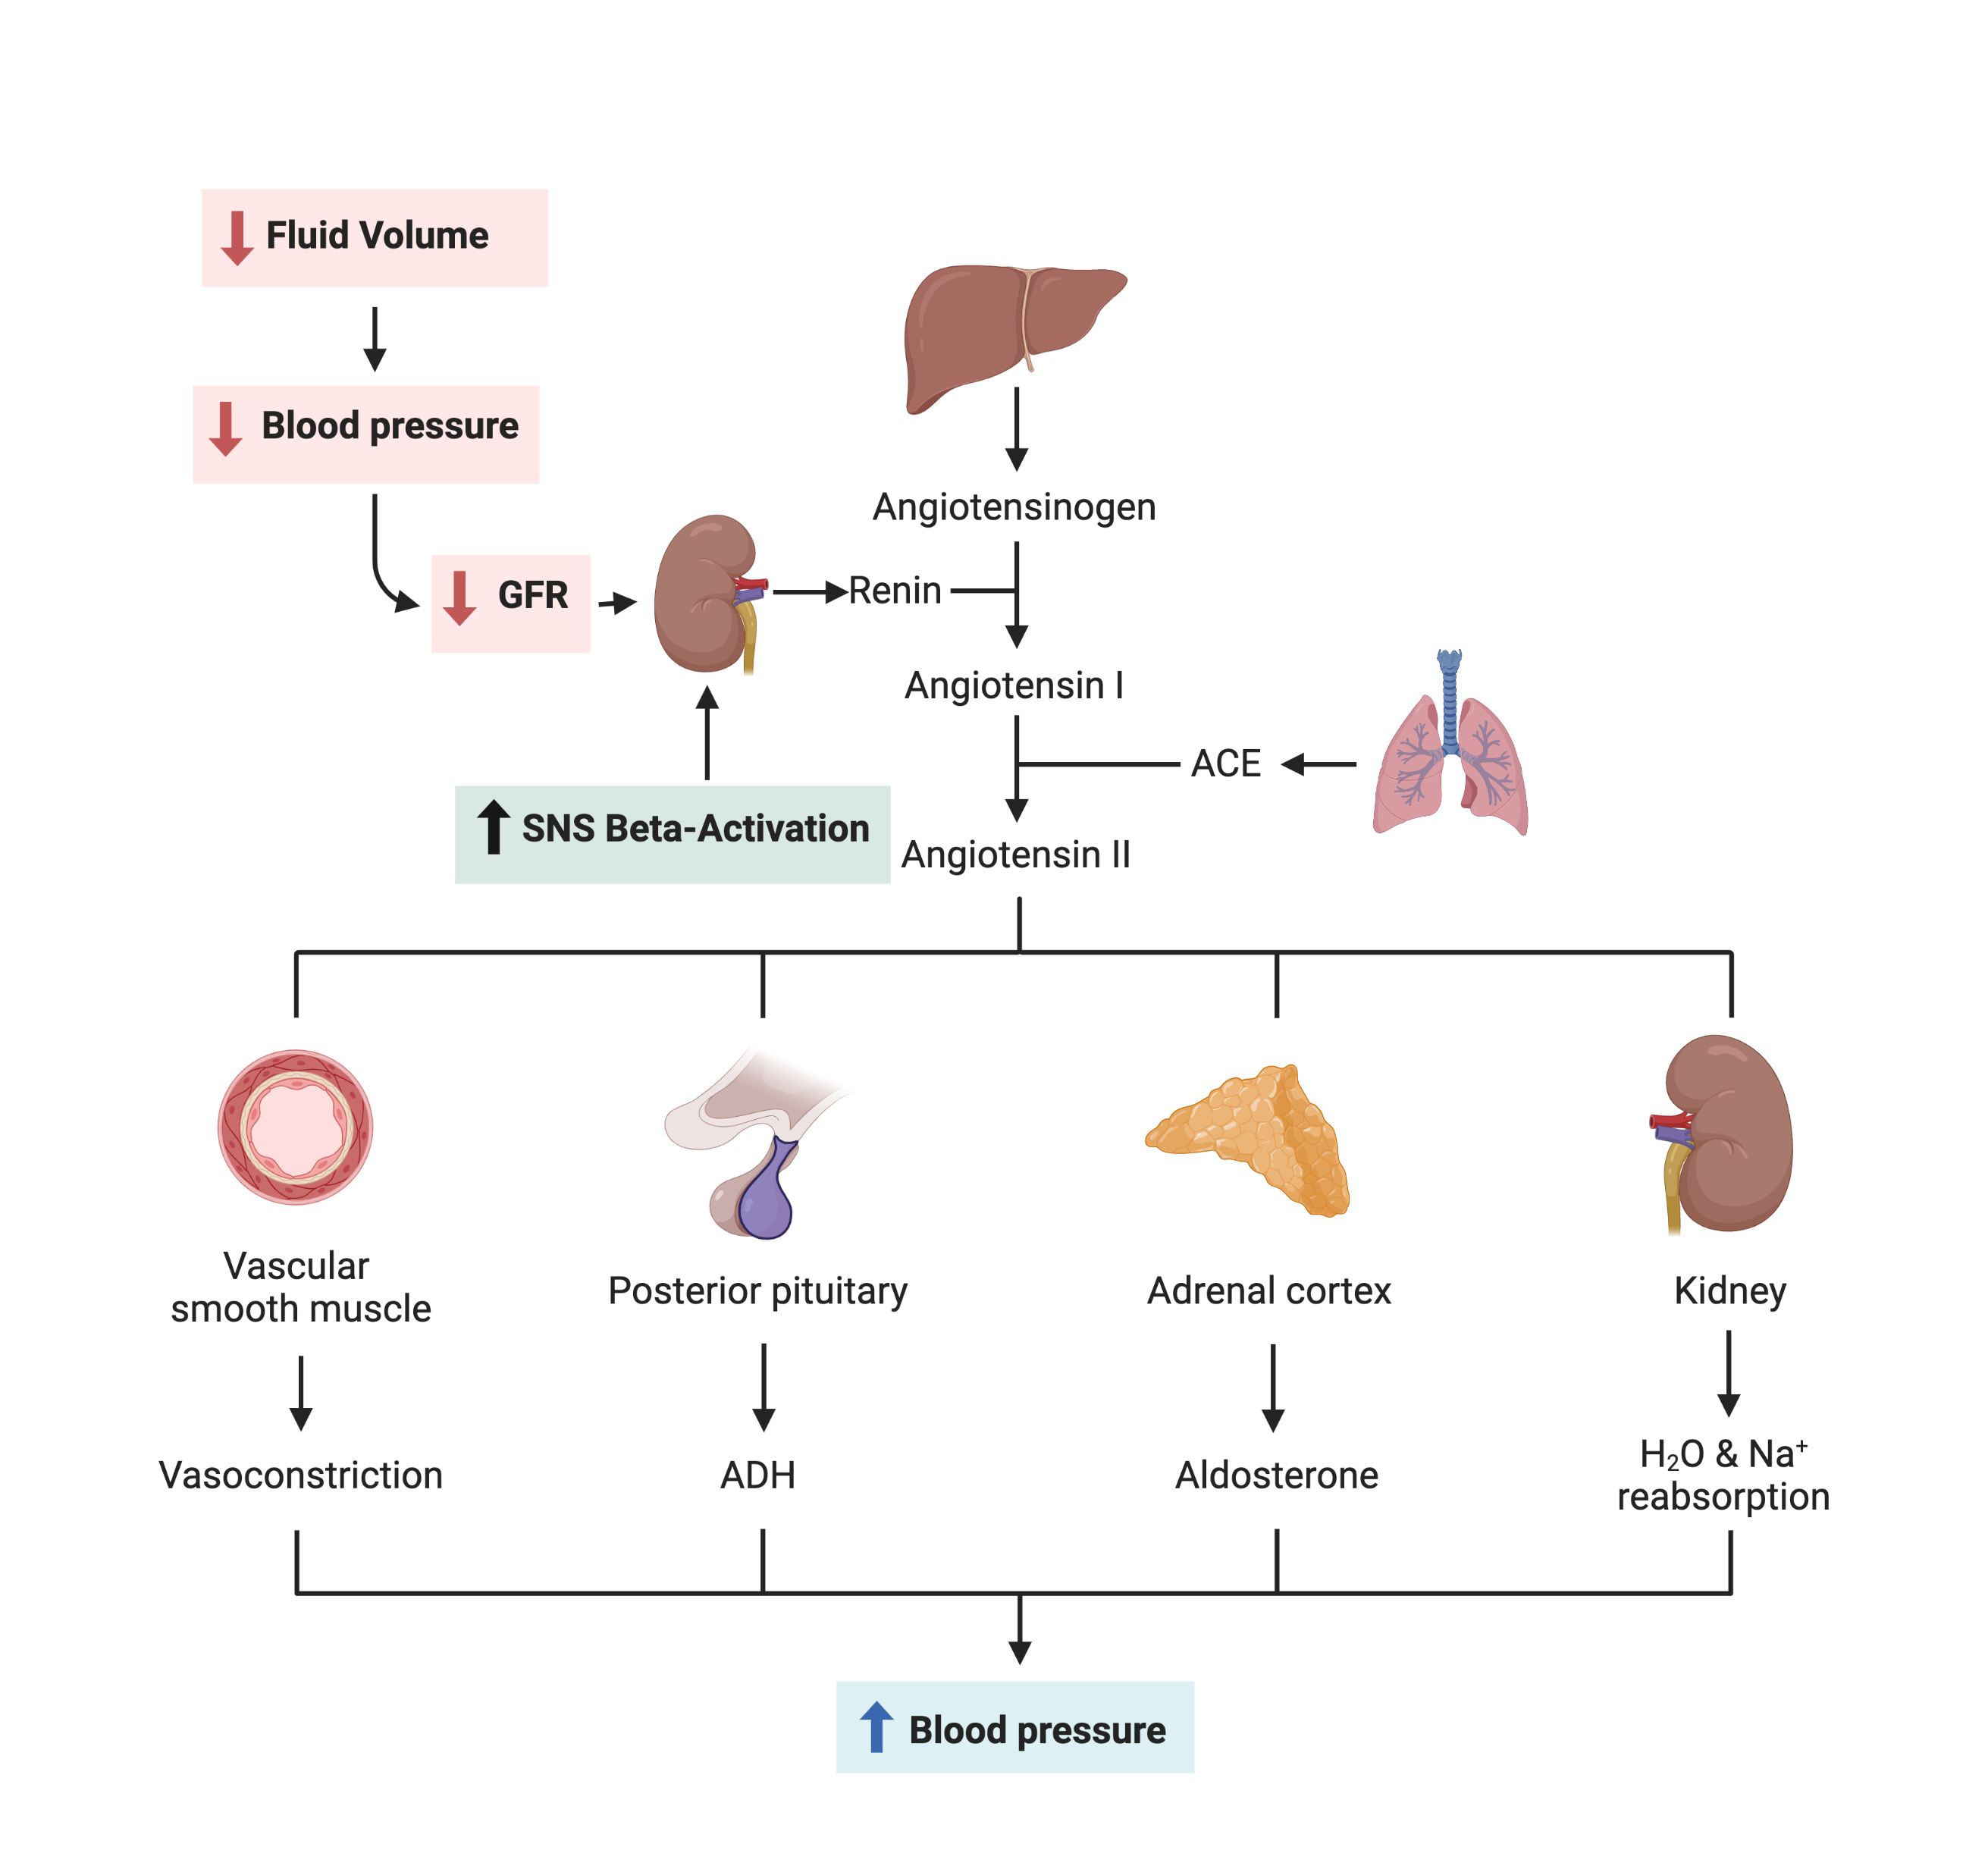
\includegraphics[width=1\linewidth]{./figure/raas.png}
    \caption{Renin Angiotensin System \footnotesize{(Created with BioRender.com)}}
    \label{fig:raas}
\end{figure}

\paragraph{RAAS Gone Wrong - Heart Failure \& ACE-Inhibition}

The events of RAAS depicted in Figure \ref{fig:raas} can go wrong. With chronic heart failure (HF) there can be reduced BP, or even with preserved BP but lower cardiac output, reduced RBF and GFR, that promotes the secretion of renin by the kidneys. In the context of HF, RAAS increases return of blood to the heart (preload) due to an increased vascular volume. The increased preload adds additional burden to an already failing heart. RAAS also increases the load that the heart must pump against (afterload) due to an increased blood pressure and systemic vasoconstriction. The increased afterload also adds additional burden to an already failing heart. The result tends to be a further reduction in cardiac output and GFR which promotes more renin secretion. This positive feedback loop is far from positive for the health of the individual with HF. In such situations the best course of action for restoring stability is a class of medication referred to a ACE-Inhibitors (ACE-I, i.e. captopril, lisinopril, enalapril) that block the enzyme at converts angiotension I to angiotensin II. ACE-I are also a preferred treatment for HTN (high blood pressure). Rather than forcing diuresis (as a diuretic does, which can create hypokalemia), they prevent anti-diuresis. Anti-anti diuresis is a gentle and physiologically stable approach to diuresis that prevents one of the several deleterious responses to reduced GFR due to HF. The therapuetic benefit of ACE-I goes beyond preventing anti-diuresis and includes reducing the release of aldosterone, and preventing angiotensin II from directly vasoconstricting blood vessels (increasing total peripheral resistance (TPR) and diastolic blood pressure (DBP)), and directly resulting in water and $Na^+$ reabsorption.

\paragraph{Overall Integration of Renal Mechanisms and Arterial Pressure}

Figure \ref{fig:integrated_renal_bp} is a directed graph that depicts the closed loop integration of renal and circulatory systems through the renal regulation of blood volume, and the arterial pressure influence over renal excretion. 

\begin{figure}[!h]
    \centering
    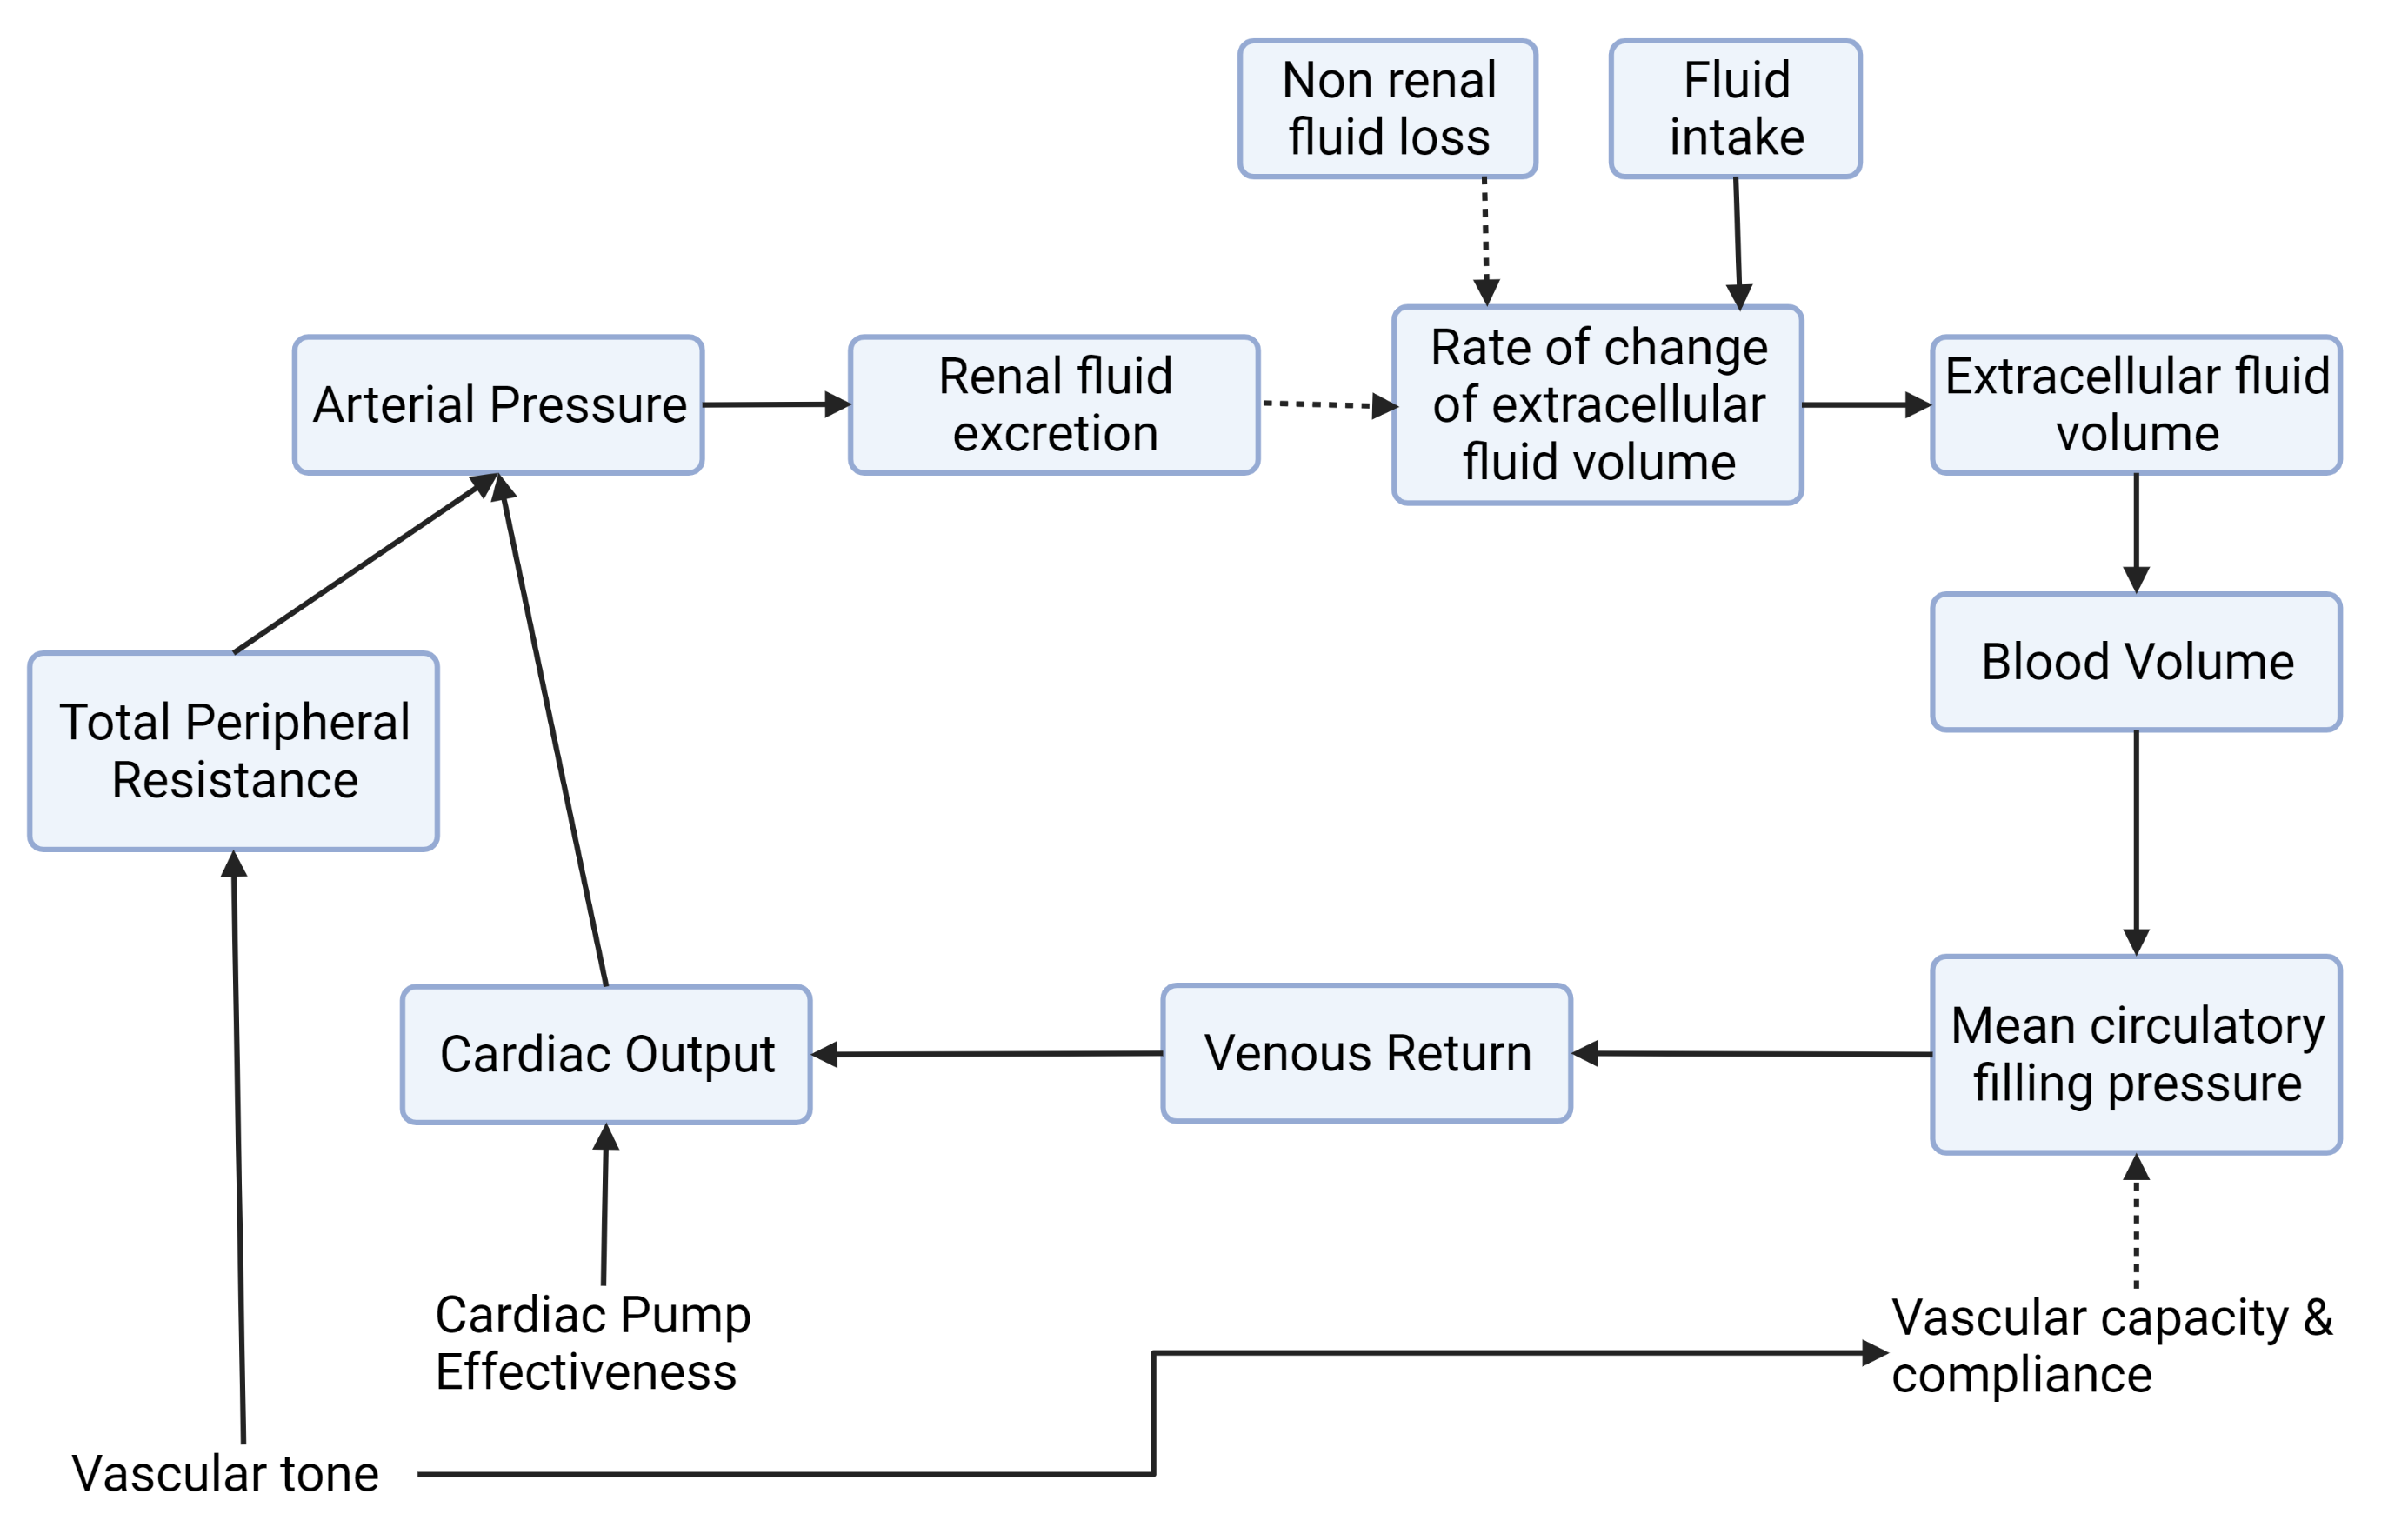
\includegraphics[width=1\linewidth]{./figure/integrated_renal_bp.png}
    \caption{Integration of Renal Mechanisms with Arterial Pressure  \footnotesize{(Modified from \cite{hall_guyton_2020} with BioRender.com)}}
    \label{fig:integrated_renal_bp}
\end{figure}

The variables in Figure \ref{fig:integrated_renal_bp} are familiar other than he mean circulatory filing pressure ($P_{mcf}$). $P_{mcf}$ is a variable created by Guyton in a model of renal blood pressure regulation \cite{rothe_mean_1993}. $P_{mcf}$ is defined as the mean vascular pressure that exists with a stop in cardiac output and distribution of blood until all pressures are the same throughout the system. It is related to the fullness of the circulatory system. A change in $P_{mcf}$ is a useful index of a change in overall venous smooth muscle tone if the blood volume is not changed. $P_{mcf}$ estimates the pressure in the small veins and venules, which contain most of the blood and account for most of the compliance. In total, $P_{mcf}$ provides an estimate of the pressure that determines the rate of flow returning to the heart, independent of cardiac output.



\subsubsection{Neuroendocrine Influence of the Vascular System}

\paragraph{Neural Input}

The autonomic neuroendocrine system influences the heart via direct neural connections and through circulating hormones. It is important to keep in mind that the SA node is the pacemaker. The neuroendocrine input influences, but does not pace, the heart. The multitude of competing external influences to the pacing of HR is one of the reasons for the phenomenon known as HR variability (HRV). 

The parasympathetic (cholinergic) system has direct neural input through the cardiac branch of the vagal nerve (Cranial Nerve X). Vagal nerve activity generally decelerates cardiac function, thus decreasing HR, speed of the conduction wave of excitation and to a lesser extent contractility. The right vagus nerve stimulates primarily the SA node and affects rate, whereas the left vagus nerve stimulates primarily the AV node and affects AV conduction. Note that parasympathetic neural input does not influence EDV. However, EDV can influence parasympathetic neural input (see the Bainbridge reflex below).

Sympathetic (adrenergic) system neural input is through the thoracolumbar sympathetic system and increases HR and augments contractility, thus increasing cardiac function. The sympathetic nervous system also has connections to the peripheral vascular (arteries, arterioles, veins, venuoles). Therefore the sympathetic nervous system can change peripheral resistance, which changes vascular pressure and can alter venous return. Therefore, sympathetic influences can influence EDV. 

Autonomic coordination: It should be noted that skeletal muscle activity has an influence over venous return. When the activity of these the sympathetic nervous system is coordinated with physical activity there is an increase in EDV due to increased skeletal muscle activity that compliments the other sympathetic influences. With the lack of sympathetic activity, and an increase in parasympathetic activity there is a decrease in EDV due to decreased skeletal muscle activity that compliments the other parasympathetic influences. 

\paragraph{Endocrine Input}
In response to physical activity or stress, the sympathetic nervous system releases catecholamines (epinephrine and norepinephrine) from the adrenal cortex of the adrenal glands which increases HR, contractility, and total peripheral resistance for a net effect of increased cardiac function. Increased TPR has the effect of helping to facilitate venous return which then contributes to EDV. The endocrine influence of the sympathetic nervous system provides a more efficient mechanism for fight/flight signaling since hormones, once circulating in the blood, continue to exert their influence. 

\paragraph{Local Input}
Tissue pH, concentration of carbon dioxide ($CO_2$), concentration of oxygen ($O_2$), and metabolic products (e.g., lactic acid) can affect vascular tone. During exercise, increased levels of $CO_2$, decreased levels of $O_2$, decreased pH, and increased levels of lactic acid at the tissue level dilate local blood vessels and therefore increase $\dot{Q}$ distribution to that area. The number of arterioles dilating due to local input is related to the drop in peripheral resistance and influences both venous return and the BP response, which then influences cardiac pump function. 

\subsubsection{Cardiac Reflexes}
Cardiac reflexes influence HR and contractility and can be divided into four general categories: baroreflex (pressure), Bainbridge reflex (stretch), chemoreflex (chemical reflex), ergoreflex (ergoreceptors). 

\paragraph{Baroreflex}

The baroreflex is activated through a group of mechanoreceptors located in the heart, great vessels, and intrathoracic and cervical blood vessels. These mechanoreceptors are most plentiful in the walls of the internal carotid arteries. Mechanoreceptors are sensory receptors that are sensitive to mechanical changes, such as pressure and stretch. Increased activity in the mechanoreceptors by high pressures increases vagal output and decreases sympathetic output. This chain of events results in vasodilation, decreased HR, and decreased contractility. The net effect is lower HR and SV, which reduce $\dot{Q}$ and therefore BP. Reduction in activity in the mechanoreceptors by low pressure results decreases vagal output and increases sympathetic output. This chain of events results in vasoconstriction, increased HR, and increased contracility. The net effect is higher HR,  SV (as compared to lower sympathetic activity), which increase $\dot{Q}$ and therefore BP. The baroreflex is a quintesstential homeostatic negative feedback system - elevated BP promotes reduced BP, and reduced BP promotes elevated BP. It is the fast acting regulator of BP during body position changes that prevents syncope (loss of consciousness) during orthostatic challenges  (moving from supine to sit or standing).
Dysfunction of any part of the baroreflex can result in orthostatic intolerance (hypotension with position changes) that can include syncope. The baroreflex may also be involved in the poorly coordinated response to orthostatic challenges displayed in postural orthostatic tachycardia syndrome (POTS) where BP does not drop with position changes, but HR increases and is sustained at a high level for longer, which when utilized alone to regulate BP is not the most efficient of effective mechanism.  













\section{Circulation}

\subsection{Systemic Circulation = Cardiac Output}
$\dot{Q}$ is the quantity of blood circulated through the systemtic vessels by the heart in 1 minute. Regional demands for tissue perfusion (based on local metabolic needs) compete for systemic circulation, and total $\dot{Q}$ adjusts to meet these demands. Adjustment to $\dot{Q}$ occurs with changes in heart rate (HR—chronotropic) or stroke volume (SV—inotropic). Normal resting $\dot{Q}$ is approximately 4 to 8 liters per minute (L/min), with a resting HR of 70 beats per minute (bpm); resting SV is approximately 71 mL/beat. The maximum value of $\dot{Q}$ represents the functional capacity of the circulatory system to meet the demands of physical activity.

\paragraph{Cardiac Index}
$\dot{Q}$ also can be described relative to body mass as the cardiac index (CI), the amount of blood pumped per minute per square meter of body mass. Normal CI is between 2.5 and 4.2 $L/min/m^2$. This wide normal range makes it possible for $\dot{Q}$ to decline by almost 40\% and still remain within the normal limits. Although several factors interrupt a direct correlation between CI and functional aerobic capacity,  CI below 2.5 $L/min/m^2$ represents a marked disturbance in cardiovascular performance and is always clinically relevant.

\paragraph{Distribution of Systemic Circulation}
The distribution of all systemic circulation starts with the aorta (See Figure \ref{fig:Cardiac_Anatomy}). Systemic circulation is affected by total peripheral resistance (TPR), which is the resistance to circulation by the force created by the aorta and arterial system. As depicted in Equation \ref{Poiseuille}, the two factors that contribute to resistance are (1) vasomotor tone, in which vessels dilate and constrict to change their radius (and compliance); and (2) blood viscosity, in which greater pressure is required to propel thicker blood. TPR, also called systemic vascular resistance, and $\dot{Q}$ influence BP (See Equation \ref{BP}. 

\subsection{Cardiac Circulation}

The major coronary arteries include the left coronary (LCA) which quickly branches into the left anterior descending (LAD) and left circumflex (LCx); and the right coronary artery RCA) (See Figure \ref{fig:Cardiac_Circulation}). LAD distributes the anterior wall of both ventricles (L > R) including the septum. LCx the left lateral and posterior walls. LAD and LCx join for distribution in the inferior myocardium. RCA distributes to the anterolateral, lateral, posterior and inferior RV. The RCA and LCA are the first two vessels off of the aorta. Blood is pumped to these large superficial coronary arteries during ventricular systole. At this time, myocardial contraction limits the flow of blood to the myocardium; therefore myocardial tissue is perfused during diastole.

\begin{figure}[!h]
    \centering
    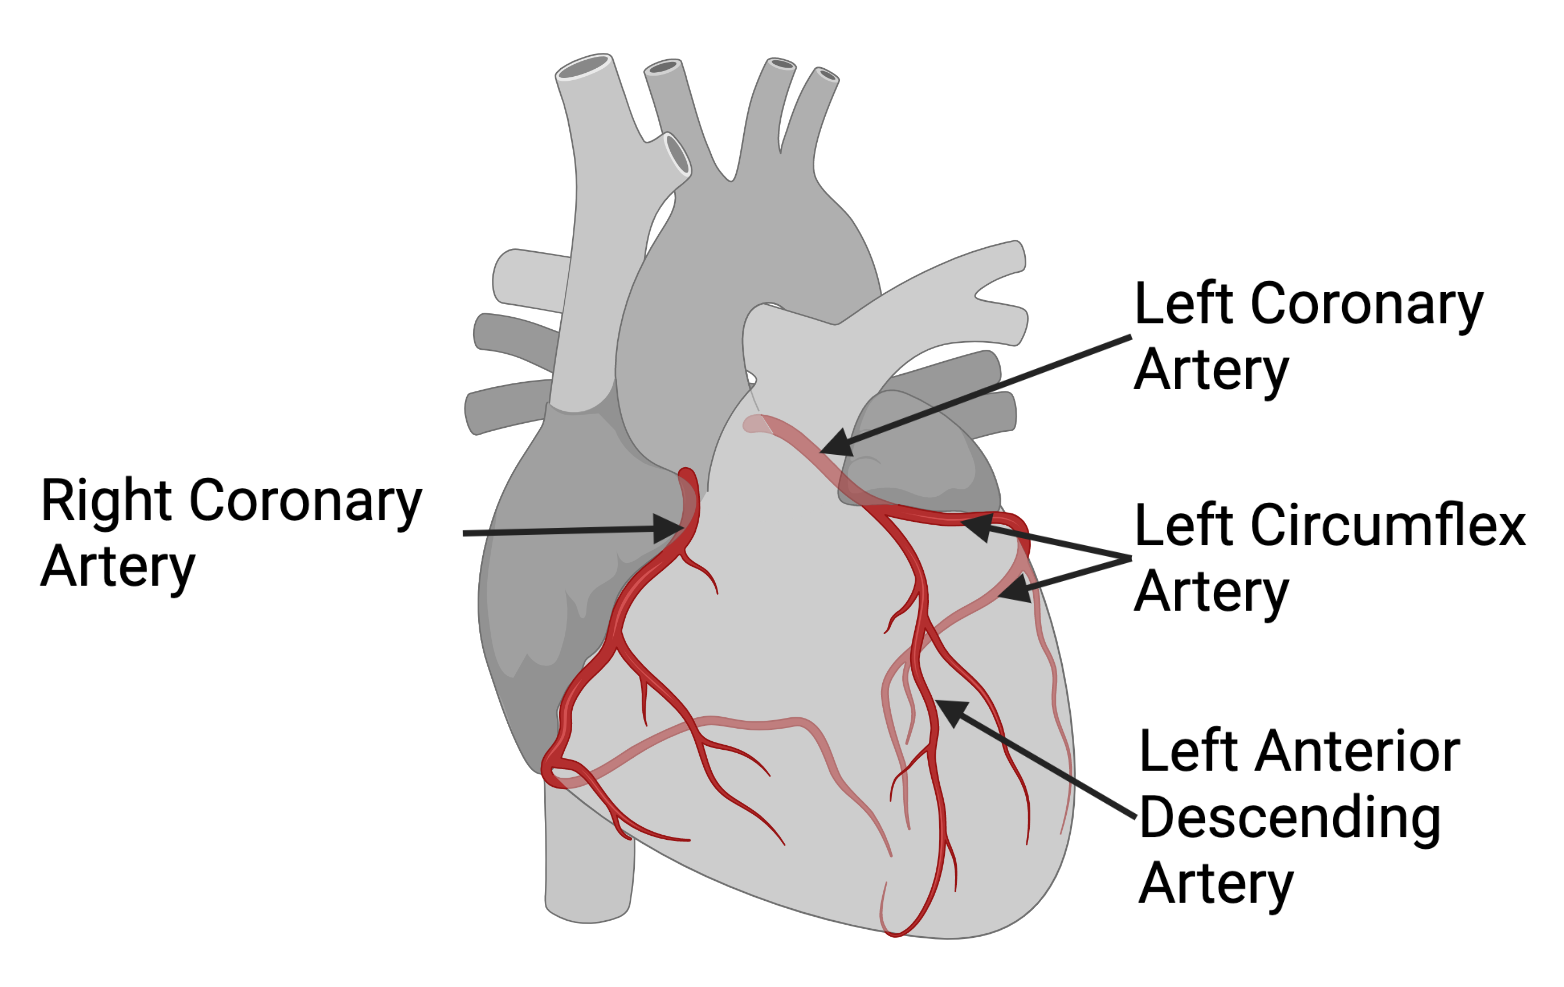
\includegraphics[width=0.5\linewidth]{./figure/Cardiac_Circulation.png}
    \caption{Cardiac Circulation \footnotesize{(Created with BioRender.com)}}
    \label{fig:Cardiac_Circulation}
\end{figure}

\subsection{Pulmonary Circulation}
For overall balanced systemic circulation, where blood returns to the RA and leaves through the LV, the pulmonary circulation must equate to the systemic circulation. Therefore, all prior discussions about $\dot{Q}$, apply to the pulmonary circulation. One primary difference between the pulmonary and systemic circulation is the resistance. Resistance is much lower in the pulmonary circulation. Pulmonary circulation has much less length - recall from Equation \ref{resistance} that length is directly proportional to resistance. With less resistance the RV does not need to exert as much pressure (or tension) to produce circulation through the pulmonary circuit. Therefore, while the volume (L/min) through the pulmonary and systemic circulations are the same, the pressures are different by an order of magnitude. The Pulmonary Artery Pressure (PAP) is approximately 15-25/0-5 mmHg during RV systole / RV diastole. Factors regulating the pulmonary circulation are discussed in Chapter \ref{chp:respiration} on Blood Gases.

\section{Cardiovascular Vital Signs}

\subsubsection{Palpation of Pulses} 
Palpation of pulses is an important component of a physical examination and can be used to evaluate and identify the following:

\begin{itemize}
\item Circulation quality
\item Pulse rate and rhythm
\end{itemize}

\paragraph{Circulation Quality}

Pulse are pressure waves through the circulation that are related to both blood pressure and local circulation. Weak pulses can indicate either low blood pressure (overall) or poor circulation that particular region of the body. For example, a weak pulse in the right radial artery but not the left radial artery most likely indicates a local circulation problem in the left UE but not the right. Whereas a weak pulse in all extremities is most likely a low blood pressure overall. A strong, or bounding, pulse can indicate a high blood pressure overall, or a high blood pressure in a particular area. Bounding pulses can also indicate vascular abnormalities such as aneurysms (for example a bounding abdominal pulse is a sign of a descending aortic aneurysm).

\paragraph{Heart Rate \& Rhythm}

Pulses are correlated with heart rate (cardiac cycle) and rhythm. When palpating a pulse to obtain HR, counting the pulse rate for 15 seconds and multiplying by 4 is sufficient with normal rates and rhythms. If rates are faster than 100 bpm or slower than 60 bpm, palpate the pulse for 60 seconds. If the rhythm is irregularly irregular (e.g., during AFib) or regularly irregular (e.g., PACs or PVCs), perform auscultation of heart sounds to identify the apical HR for a full minute. In these cases, palpation of pulse cannot substitute for ECG analysis to monitor the patient’s rhythm, but it may alert the therapist to the onset of these abnormalities.

Use caution in palpating pulses because manual pressure on the carotid sinus may cause baroreflex drops in heart rate (HR), blood pressure (BP), or both. In all pulse palpation situations the examiner should start with light pressure and gradually increase pressure until a pulse is felt, and to not exert more pressure than required to feel the pulse.

Some people can feel a pulse in their thumb, therefore it is generally advised to not use the thumb to palpate a pulse.

HR is the primary means of determining the exercise intensity level for patients who are not taking beta-blockers or who have rate-responsive pacemakers. HR combined with blood pressure (RPP) is the most appropriate approach to determine exercise intensity in any patient with a known ischemic threshold (even if they are on beta-blockers).

\begin{itemize}
\item A linear relationship exists between HR and work.
\item In general, a 20- to 30-beat increase from the resting value during activity is a safe intensity level in which a patient can exercise.
\item If a patient has undergone an exercise stress test during the hospital stay, a percentage (e.g., 60\%–80\%) of the maximum HR achieved during the test can be calculated to determine the exercise intensity.
\item An example of a disproportionate HR response to low-level activity (bed or seated exercises or ambulation in room) is an HR of more than 120bpm or less than 50bpm.
\item Heart rate recovery (HRR), provides an indication of reduced parasympathetic activity and an indicator of all-cause mortality, can be used to document improvement of tolerance to functional demands. HRR is the absolute difference between peak HR achieved with exercise minus the HR at 60 seconds after the completion of exercise (HRR 60 sec).  An abnormal HRR at 1 minute, after a treadmill test, is reported to be a decrease of 12 bpm or less with a cool-down period and less than 18 bpm without a cool-down period \cite{collins_cardiac_2019}.
\item When prescribing activity intensity for a patient taking beta-blockers, consider that HR should not exceed 20 beats above the resting HR. If RPP for the patient's ischemic threshold is known, then the RPP should not be allowed to increase to the ischemic threshold.
\item If prescribing an activity intensity, with use of HR, for patients with an automatic implantable cardiac defibrillator (AICD), remember that the exercise target HR should be 20 to 30 beats below the threshold rate on the defibrillator.
\item HR should not be used to prescribe exercise status post heart transplantation secondary to denervation of the heart during transplantation.
\item Baseline HR and recent changes in medications always should be considered before beginning an exercise session.
\end{itemize}

\subsubsection{Blood Pressure}

Blood pressure is critical to circulation and a primary variable utilized to help regulate cardiac output. Low blood pressure (and low PP) is problematic because it compromises circulation and may indicate hemodynamic compromise due to cardiac (reduced cardiac output), vascular (reduced peripheral resistance) or blood volume problems. High blood pressure can create immediate health care emergencies by placing blood vessels under too much pressure; or cardiac emergencies by causing ischemia (high RPP and myocardial $O_2$ demand), or heart failure (increased afterload). Long term increased high blood pressure (hypertension) leads to long term changes in the heart (left ventricular hypertrophy, fibrosis of the atria and ventricles that makes the heart more susceptible to arrhythmias, or valve dysfunction). Hypertension is a silent killer since many individuals have no idea they have it - which is one of the reasons for the APTA Academy of Cardiovascular and Pulmonary Physical Therapy's "Vitals are Vital" campaign to encourage all physical therapists in all settings to make sure they routinely examine vitals signs in all clients.

Measurement of BP with a sphygmomanometer (cuff) and auscultation is an indirect, noninvasive measurement of the force exerted against the arterial walls during ventricular systole (SBP) and during ventricular diastole (DBP). BP is affected by total peripheral resistance (blood volume, radius and compliance of arterial walls) and $\dot{Q}$. Table \ref{table:BP_Ranges} includes normal BP ranges. 

\begin{table}[h!]
\centering
\begin{tabular}{||c c c ||} 
 \hline
 Ranges & Systolic (mmHg) & Diastolic (mmHg) \\ [0.5ex] 
 \hline\hline
Age 8 years & 85-114  & 52-85  \\ 
Age 12 years & 95-135  & 58-88   \\
Adult & $<$ 120   & $<$ 80   \\
Elevated (Adult) & 120-129   & $<$ 80  \\
Stage 1 Hypertension & 130-139  & 80-89   \\
State 2 Hypertension & $\geq$ 140 &  $\geq$ 90 \\ [1ex] 
 \hline
\end{tabular}
\caption{Blood Pressure Ranges, Modified from \cite{collins_cardiac_2019}}
\label{table:BP_Ranges}
\end{table}

Occasionally, BP measurements can be performed only on certain limbs secondary to the presence of such conditions as a percutaneously inserted central catheter, arteriovenous fistula for hemodialysis, blood clots, or lymphedema (e.g., status post mastectomy). 

BP of the upper extremity should be measured in the following manner \cite{collins_cardiac_2019}:

\begin{enumerate}
\item Check for posted signs, if any, at the bedside that indicate which arm should be used in taking BP. BP variations of 5 to 10 mmHg between the right and left upper extremity are considered normal. Patients with arterial compression or obstruction may have differences of more than 10 to 15 mmHg.
\item Use a properly fitting cuff. The inflatable bladder should have a width of approximately 40\% and length of approximately 80\% of the upper arm circumference.
\item Position the cuff 2.5 cm above the antecubital crease.
\item Rest the relaxed arm at the level of the heart.
\item To determine how high to inflate the cuff, palpate the radial pulse, inflate until no longer palpable, and note the cuff inflation pressure. Deflate the cuff. This is an estimate of the systolic pressure. But this method cannot be utilized to obtain a diastolic pressure.
\item Place the bell of the stethoscope gently over the brachial artery.
\item Reinflate the cuff to 30 to 40 mmHg greater than the value in step 5. Then slowly deflate the cuff. Cuff deflation should occur at approximately 2 to 3 mmHg per second.15
\item Listen for the onset of tapping sounds, which represents circulation returning to the brachial artery. This is the SBP.
\item As the pressure approaches diastolic pressure, the sounds will become muffled and in 5 to 10mmHg will be completely absent. These sounds are referred to as Korotkoff sounds (See Table \ref{Korotkoff}).
\end{enumerate}

\begin{table}[h!]
\centering
\begin{tabular}{||c c c ||} 
 \hline
 Phase & Korotkoff Sound & Indicates \\ [0.5ex] 
 \hline\hline
1  & First sound, faint tapping  & Systolic pressure (circulation through compressed artery)  \\ 
2  & Blowing or swishing sound  & Blood is increasing   \\
3 & Distinct tapping   & Circulation is increasing   \\
4 & Muffled  & Diastolic pressure in certain situations$^a$\\
5 & Disappearance  & Diastolic pressure in adults   \\ [1ex] 
 \hline
\end{tabular}
\caption{Blood Pressure Ranges ($^a$ \footnotesize{Phase 4 represents DBP in children, and adults that are exercising, pregnant or with hyperthyroid conditions})(Modified from \cite{bickley_bates_2012})}a
\label{Korotkoff}
\end{table}

\paragraph{Systolic Blood Pressure / Palp}

In situations when it is difficult to auscultate or to obtain a distinct diastolic blood pressure reading (DBP), the palpation method may be utilized and blood pressure is noted as systolic blood pressure (SBP)/Palp. This is the same procedure utilized in Step 5 to determine how high to pump the cuff for a full measurement of blood pressure without having to over inflate the cuff.


\subsection{Physical Therapy Considerations}
\begin{itemize}
\item Recording pre exertion, para exertion, and post exertion BP is important for identification of BP responses to activity. During recovery from exercise, blood vessels dilate to allow for greater circulation to muscles. In cardiac-compromised or very deconditioned individuals, total $\dot{Q}$ may be unable to support this increased flow to the muscles and may lead to decreased output to vital areas, such as the brain.
\item If you are unable to obtain BP on the arm, the thigh is an appropriate alternative, with auscultation at the popliteal artery.
\item Falsely high readings occur if the cuff is too small or applied loosely or if the brachial artery is lower than the heart level.
\item Evaluation of BP and HR in different postures can be used to monitor orthostatic hypotension with repeat measurements on the same arm 1 to 5 minutes after position changes.
\item The same extremity should be used when serial BP recordings will be compared for an evaluation of hemodynamic response.
\item A BP record is kept on the patient’s vital sign flow sheet. This is a good place to check for BP trends throughout the day and, depending on your hospital’s policy, to document BP changes during the therapy session.
\item An auscultatory gap is the disappearance of sounds between phase 1 and phase 2 and is common in patients with high BP, venous distention, and severe aortic stenosis. Its presence can create falsely low SBPs if the cuff is not inflated enough (prevented by palpating for the disappearance of the pulse before measurement), or falsely high DBPs if the therapist stops measurement during the gap (prevented by listening for the phase 3 to phase 5 transitions).
\item In general there is a lower SBP, higher DBP, and lower workload at any given submaximal HR during arm exercise compared with leg exercise \cite{dias_differences_2022}
\item A clearly disproportionate response to exercise includes SBP decrease of 10 mmHg below the resting value, a hypertensive systolic response of greater than 200 mmHg, or a hypertensive diastolic response of greater than 110 mmHg. A normotensive systolic blood response should increase 5 to 12 mmHg per increase in metabolic equivalents (METs).\footnotemark\footnotetext{One MET is approximately 3.5 ml/kg/min of oxygen consumption.}
\item If the patient is on a pacemaker that does not have rate modulation, BP response can be used to gauge intensity. 
\end{itemize}



\section{Summary}

Circulation supports micro-circulation and therefore ECF. Circulation is measured by $\dot{Q}$ and tends to be regulated by monitoring BP through the adjustment of HR (chronotropy), cardiac contractility (inotropy) and TPR. Cardiac muscle includes several characteristics required for its unique role in circulation. Cardiac muscle tension, excitation and regulation support circulation and pressure regulation. Excitation of cardiac muscle can be recorded with the ECG and offers insights into several abnormalities of conduction as well as myocardial ischemia. Monitoring ECG, BP and HR provide physical therapists with non-invasive insights, that when combined with an understanding of circulatory physiology, provide useful information when working with clients both with and without conditions that directly affect the circulation.

\subsection{Circulation Summary}

Throughout this chapter the cardiac and vascular factors that influence circulation are covered at length. These factors all ultimately influence the variables in the equations of this section. They ultimately influence the pressure gradient generated by cardiac muscle tension and arteriole radius which influence volume, pressure, compliance and resistance to flow. Regulation BP is a major topic due to its centrality in the regulation of circulation. Regulation of BP is also discussed in Chapter \ref{chp:filtration_reabsorption_secretion} on Renal Clearance since having the right blood volume is an important aspect of maintaining BP and circulation.

\subsection{Next Step}

With a deeper understanding of mass balance we can now proceed to the mass balance of oxygen and carbon dioxide in the next two chapters. Chapter \ref{chp:respiration} on Respiration focuses on gas exchange between the alveoli and blood. Chapter \ref{chp:ventilation} on Ventilation focuses on air exchange between the environment and the alveoli (breathing).

\printbibliography[heading=subbibintoc]